% Options for packages loaded elsewhere
\PassOptionsToPackage{unicode}{hyperref}
\PassOptionsToPackage{hyphens}{url}
%
\documentclass[
]{article}
\usepackage{amsmath,amssymb}
\usepackage{lmodern}
\usepackage{iftex}
\ifPDFTeX
  \usepackage[T1]{fontenc}
  \usepackage[utf8]{inputenc}
  \usepackage{textcomp} % provide euro and other symbols
\else % if luatex or xetex
  \usepackage{unicode-math}
  \defaultfontfeatures{Scale=MatchLowercase}
  \defaultfontfeatures[\rmfamily]{Ligatures=TeX,Scale=1}
\fi
% Use upquote if available, for straight quotes in verbatim environments
\IfFileExists{upquote.sty}{\usepackage{upquote}}{}
\IfFileExists{microtype.sty}{% use microtype if available
  \usepackage[]{microtype}
  \UseMicrotypeSet[protrusion]{basicmath} % disable protrusion for tt fonts
}{}
\makeatletter
\@ifundefined{KOMAClassName}{% if non-KOMA class
  \IfFileExists{parskip.sty}{%
    \usepackage{parskip}
  }{% else
    \setlength{\parindent}{0pt}
    \setlength{\parskip}{6pt plus 2pt minus 1pt}}
}{% if KOMA class
  \KOMAoptions{parskip=half}}
\makeatother
\usepackage{xcolor}
\IfFileExists{xurl.sty}{\usepackage{xurl}}{} % add URL line breaks if available
\IfFileExists{bookmark.sty}{\usepackage{bookmark}}{\usepackage{hyperref}}
\hypersetup{
  pdftitle={SCMA329 Practical Mathematical Financial Modeling},
  pdfauthor={Pairote Satiracoo},
  hidelinks,
  pdfcreator={LaTeX via pandoc}}
\urlstyle{same} % disable monospaced font for URLs
\usepackage[margin=1in]{geometry}
\usepackage{longtable,booktabs,array}
\usepackage{calc} % for calculating minipage widths
% Correct order of tables after \paragraph or \subparagraph
\usepackage{etoolbox}
\makeatletter
\patchcmd\longtable{\par}{\if@noskipsec\mbox{}\fi\par}{}{}
\makeatother
% Allow footnotes in longtable head/foot
\IfFileExists{footnotehyper.sty}{\usepackage{footnotehyper}}{\usepackage{footnote}}
\makesavenoteenv{longtable}
\usepackage{graphicx}
\makeatletter
\def\maxwidth{\ifdim\Gin@nat@width>\linewidth\linewidth\else\Gin@nat@width\fi}
\def\maxheight{\ifdim\Gin@nat@height>\textheight\textheight\else\Gin@nat@height\fi}
\makeatother
% Scale images if necessary, so that they will not overflow the page
% margins by default, and it is still possible to overwrite the defaults
% using explicit options in \includegraphics[width, height, ...]{}
\setkeys{Gin}{width=\maxwidth,height=\maxheight,keepaspectratio}
% Set default figure placement to htbp
\makeatletter
\def\fps@figure{htbp}
\makeatother
\setlength{\emergencystretch}{3em} % prevent overfull lines
\providecommand{\tightlist}{%
  \setlength{\itemsep}{0pt}\setlength{\parskip}{0pt}}
\setcounter{secnumdepth}{5}
\usepackage{booktabs}
\usepackage{amsthm}
\usepackage{LectureNoteMacro}
\usepackage{bbm}
\usepackage{mathtools}
\usepackage{tikz}
\makeatletter
\def\thm@space@setup{%
  \thm@preskip=8pt plus 2pt minus 4pt
  \thm@postskip=\thm@preskip
}
\makeatother
\ifLuaTeX
  \usepackage{selnolig}  % disable illegal ligatures
\fi
\usepackage[]{natbib}
\bibliographystyle{plainnat}

\title{SCMA329 Practical Mathematical Financial Modeling}
\author{Pairote Satiracoo}
\date{2021-09-04}

\usepackage{amsthm}
\newtheorem{theorem}{Theorem}[section]
\newtheorem{lemma}{Lemma}[section]
\newtheorem{corollary}{Corollary}[section]
\newtheorem{proposition}{Proposition}[section]
\newtheorem{conjecture}{Conjecture}[section]
\theoremstyle{definition}
\newtheorem{definition}{Definition}[section]
\theoremstyle{definition}
\newtheorem{example}{Example}[section]
\theoremstyle{definition}
\newtheorem{exercise}{Exercise}[section]
\theoremstyle{definition}
\newtheorem{hypothesis}{Hypothesis}[section]
\theoremstyle{remark}
\newtheorem*{remark}{Remark}
\newtheorem*{solution}{Solution}
\begin{document}
\maketitle

{
\setcounter{tocdepth}{2}
\tableofcontents
}
\hypertarget{dates-and-date-functions}{%
\section{Dates and date functions}\label{dates-and-date-functions}}

Dates and date functions will be discussed in this section. Depending on
the system setting, the dates used in this section corresponds to the
U.S. setting, i.e.~month/day/year. Thus, 7/1/2017 corresponds to 1 July
2017.

The following date formats are recognized by Excel:

\begin{itemize}
\item
  7/1/2017, 7/1/17
\item
  7-1-2017, 7-1-17,
\item
  7-1/2017, 7-1/17,
\item
  July 1, 2017
\item
  1-Jul-2017
\end{itemize}

if the date input is without the year, then it is the date on the
current year, i.e.~7-1, 7/1, July 1, Jul 1, corresponds to 1 July 2018.

\hypertarget{inconsistent-date-entries}{%
\subsection{Inconsistent date entries}\label{inconsistent-date-entries}}

\begin{example}
\protect\hypertarget{exm:unlabeled-div-1}{}\label{exm:unlabeled-div-1}

\textbf{Example 1}. \emph{What will be the output when we enter dates by using the
following two digits for the years:}

\begin{enumerate}
\def\labelenumi{\arabic{enumi}.}
\item
  \emph{7/1/01}
\item
  \emph{7/1/60}
\end{enumerate}

\end{example}

Excel interprets two digit years between 00 and 29 as 21st century
dates, and two digit years between 30 and 99 as 20th century dates.

\hypertarget{date-serial-number}{%
\subsection{Date serial number}\label{date-serial-number}}

Excel stores dates as sequential serial numbers so that they can be used
in calculations. For example,

\begin{itemize}
\item
  1 January 1900 is serial number 1,
\item
  1 January 2018 is serial number 43101 because it is 43101 days after
  1 January 1900.
\end{itemize}

\hypertarget{date-functions}{%
\subsection{Date functions}\label{date-functions}}

The list of date functions can be seen by choosing

\textbf{Formulas \(\rightarrow\) Function Library \(\rightarrow\) Function Library \(\rightarrow\) Date \& Time}.

\begin{longtable}[]{@{}ll@{}}
\toprule
\textbf{Function} & \textbf{Description} \\
\midrule
\endhead
DATE & Returns the serial number of a particular date \\
DATEVALUE & Converts a date in the form of text to a serial number \\
DAY & Converts a serial number to a day of the month \\
DAYS & Returns the number of days between two dates \\
WEEKDAY & Converts a serial number to a day of the week \\
NETWORKDAYS & Returns the difference between two dates, excluding weekend days (Saturdays and Sundays) \\
WORKDAY & Returns a number that represents a date that is the indicated number of working days before or after a date (the starting date) \\
EDATE & Returns the serial number that represents the date that is the indicated number of months before or after a specified date \\
EOMONTH & Returns the serial number for the last day of the month that is the indicated number of months before or after a specified date \\
YEARFRAC & Returns a decimal value that represents fractional years between two dates \\
\bottomrule
\end{longtable}

For a complete list, see the date and time functions available online.
More detailed examples are also given in the Excel lab.

\hypertarget{working-with-texts}{%
\section{Working with Texts}\label{working-with-texts}}

In this section, we will see how Excel handles text strings, and how we
use text functions to modify and manipulate text strings. First, we give
a note regarding texts in Excel.

\begin{itemize}
\item
  A single cell can hold up to 32,000 characters. In case you need to
  display a lot of text in a worksheet, then use a text box (Choose
  Insert \(\Rightarrow\) Text \(\Rightarrow\) Text Box). It will be easier
  to edit texts in the text box than in cells.
\item
  Sometimes, when you download numerical data from the internet or
  database, the imported values are treated as text, i.e.~when you do
  a calculation with such data, you will get a \#VALUE error. When a
  number is not treated as a number, there will be an error indicator.
  By clinking to expand a list of options, you can then convert it to
  the number.
\item
  Another issue that you may encounter is about currency that uses
  different characters to separate thousands or decimals.
  \url{https://en.wikipedia.org/wiki/Decimal_separator}
\end{itemize}

\hypertarget{text-functions}{%
\subsection{Text functions}\label{text-functions}}

The following Excel functions can be used to modify text strings in the
format you need. Alternatively, one may extract data by using the
Convert Text To Columns Wizard (choose Data \(\Rightarrow\) Text To
Columns).

\begin{enumerate}
\def\labelenumi{\arabic{enumi}.}
\item
  RIGHT(text,{[}n{]}) returns the last \(n\) characters in a text string.
\item
  LEFT(text, {[}n{]}) returns the first \(n\) characters in a text string.
\item
  MID(text, start\_num, num\_chars) returns num\_char characters from a
  text string, starting at start\_num.
\item
  TRIM(text) removes all spaces from text except for single spaces
  between words. Use TRIM when text strings have irregular spacing.
\item
  LEN(text) returns the number of characters in a text string.
\item
  FIND(find\_text, within\_text, {[}start\_num{]}) return the location at
  or after character start\_num of the first character of find\_text in
  within\_text.
\item
  SEARCH(find\_text, within\_text, {[}start\_num{]}) has the same syntax as
  FIND, but it is not case sensitive.
\item
  SUBSTITUTE(text, old\_text, new\_text, {[}instance\_num{]}) is used to
  replace new\_text for old\_text in a text string. Here Instance\_num is
  optional. It specifies which occurrence of old\_text you want to
  replace with new\_text. If you specify instance\_num, only that
  instance of old\_text is replaced. Otherwise, every occurrence of
  old\_text in text is changed to new\_text.
\end{enumerate}

\hypertarget{character-codes}{%
\subsection{Character codes}\label{character-codes}}

Excel uses the standard ASCII character set. Therefore, each character
has its own code. For example, to get the code number of ``A'', simply
type

=CODE(``A''), which returns the code number 65.

The CHAR function reverses the role of CODE function, i.e.

=CHAR(65), which returns the letter A. The input for the CHAR function
should be a value between 1 and 255.

For the complete list of ASCII codes, please visit
\url{https://theasciicode.com.ar}

\begin{example}
\protect\hypertarget{exm:unlabeled-div-2}{}\label{exm:unlabeled-div-2}

\textbf{Example 1}. \emph{Create an Excel file to list all the first 255 ASCII
codes. It is a good idea to compare the outputs with those from the
website above.}

\end{example}

\hypertarget{determining-whether-two-string-are-identical}{%
\subsection{Determining whether two string are identical}\label{determining-whether-two-string-are-identical}}

In order to determine whether strings in cell A1 and A2 have the same
contents, we use = A1 = A2, which returns either TRUE or FALSE. Note
that the comparison is not case-sensitive.

Alternative, the function that provides an exact, case-sensitive
comparison is EXACT function.

\hypertarget{joining-two-or-more-cells}{%
\subsection{Joining two or more cells}\label{joining-two-or-more-cells}}

To join two or more cells, Excel uses an ampersand \&. For example if the
string ``the effective interest rate per annum'' is in A1 and the value of
5\% (formatted value) is in B1. Then use the formula

= A1 \& '' is '' \& B1, which returns the effective interest rate per annum
is 0.05.

A better solution is to use the TEXT function to format the value as
text as follows.

= A1 \& '' is '' \& TEXT(B1,'' 0.00\%``) , which returns the effective interest
rate per annum is 0.05.

Use \textbf{Home Format Format cells} to obtain the list of various text
formats.

For example, if A1 contains the principle of \$10,000, then

= ``The principle is'' \& TEXT(A1, '' \$\#,\#\#0''), which returns The
principle is \$10,000.

The following table gives examples that are format with TEXT function.

\begin{verbatim}
=TEXT(1234.567,"$#,##0.00")     
Currency with a thousands separator and 2 decimals, like $1,234.57. Note that Excel rounds the value to 2 decimal places.

=TEXT(TODAY(),"MM/DD/YY")
Today's date in MM/DD/YY format, like 03/14/12

=TEXT(TODAY(),"DDDD")
Today's day of the week, like Monday

=TEXT(NOW(),"H:MM AM/PM")
Current time, like 1:29 PM

=TEXT(0.285,"0.0%")
Percentage, like 28.5%

=TEXT(4.34 ,"# ?/?")
Fraction, like 4 1/3

=TRIM(TEXT(0.34,"# ?/?"))
Fraction, like 1/3. Note this uses the TRIM function to remove the leading space with a decimal value.

=TEXT(12200000,"0.00E+00")
Scientific notation, like 1.22E+07

=TEXT(1234567898,"[<=9999999]###-####;(###) ###-####")
Special (Phone number), like (123) 456-7898

=TEXT(1234,"0000000")
Add leading zeros (0), like 0001234
\end{verbatim}

The TEXT function will convert numbers to text. It is best practice to
keep your original values in one cell, and formatted number in another
cell. When you do calculation, you should refer to the cells containing
original values.

\hypertarget{interest-rate-present-values-and-cashflows}{%
\section{Interest Rate, Present Values and Cashflows}\label{interest-rate-present-values-and-cashflows}}

\hypertarget{working-with-a-single-cashflow-in-excel}{%
\subsection{Working with a single cashflow in Excel}\label{working-with-a-single-cashflow-in-excel}}

\hypertarget{how-to-calculate-the-future-value-of-a-single-cashflow}{%
\subsubsection{How to calculate the future value of a single cashflow}\label{how-to-calculate-the-future-value-of-a-single-cashflow}}

Suppose an amount \(C\) is deposited in an account that pays a fixed
interest at the rate of \(i\)\% per time units. Then after \(t\) time units,
the deposit will have accumulated to \[C (1+i)^t.\]

In Excel, the function FV calculates the future value of a single
investment (and also periodic constant payments) and a constant interest
rate.

The syntax of the function is:

\[\text{FV(rate, nper, pmt, [pv], [type])},\]

where

\begin{itemize}
\item
  rate is the interest rate per period
\item
  nper is the number of periods over which the investment is made.
\item
  pmt (used for an annuity type) is the payment made each period and
  cannot change over the life of the annuity.
\item
  pv (optional) is an additional cash flow now (time 0)
\item
  fv is an additional cash flow nper periods from now.
\item
  type (optional) is an optional argument that defines whether the
  payment is made at the start or the end of the period:

  0 - the payment is made at the end of the period;

  1 - the payment is made at the start of the period.

  If the {[}type{]} argument is omitted, it takes on the default value
  of 0.
\end{itemize}

The following timeline illustrates the cashflows used for the FV
function (assuming that the payments (pmt) are made in arrears).

\begin{figure}

{\centering 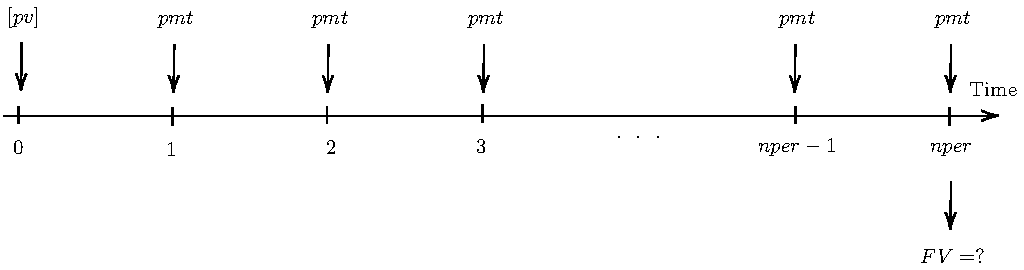
\includegraphics{SCMA329ExcelBookdownproj_files/figure-latex/tikz-ex-1} 

}

\caption{Timeline of cashflows for FV function}\label{fig:tikz-ex}
\end{figure}

\textbf{Note} For a single cash flow, we set pmt argument to be 0, as there are no
ongoing payments after the initial investment.

\begin{example}
\protect\hypertarget{exm:unlabeled-div-3}{}\label{exm:unlabeled-div-3}

\textbf{Example 1}. \emph{You plan to invest today with an interest rate of 3\% per
year effective. How much money will you accumulate at the end of 2
years?}

\end{example}

\textbf{Solution:} The accumulation of today in 2 years can be calculated by Excel as
\[\text{FV}(3\%, 2, 0, -100).\]

\hypertarget{how-to-calculate-the-present-value-of-a-single-cashflow}{%
\subsubsection{How to calculate the present value of a single cashflow}\label{how-to-calculate-the-present-value-of-a-single-cashflow}}

Similarly, the present value of a future cashflow \(C\) required at time
\(t\) time units at a fixed interest of \(i\)\% per time units can be
calculated as \[\frac{C}{(1+i)^t}.\] In Excel, the function PV
calculates the present value of a single investment (and also periodic
constant payments) and a constant interest rate. The syntax of the
function is:

\[\text{PV(rate, nper, pmt, [fv], [type])}\] where fv is an additional
cash flow nper periods from now.

\begin{example}
\protect\hypertarget{exm:unlabeled-div-4}{}\label{exm:unlabeled-div-4}

\textbf{Example 2}. \emph{How much should you deposit into the account with an
interest of 8\% so that 10 years from now its value would be ?}

\end{example}

\textbf{Solution:}
The present value of today in 10 years can be calculated by Excel as
\[\text{PV}(8\%, 10, 0, -1000).\]

\hypertarget{present-values-of-a-series-of-cashflows}{%
\subsection{Present values of a series of cashflows}\label{present-values-of-a-series-of-cashflows}}

Consider a series of cashflows defined by

\begin{enumerate}
\def\labelenumi{\arabic{enumi}.}
\item
  the times of payments (cashflows), denoted by \(t_1, t_2, \ldots,\)
  and
\item
  the amount of payments, denoted by \(C_{r}\) (in short for \(C_{t_r}\)),
  which will be paid at time \(t_r\), for \(r = 1,2, \ldots\). The amounts
  can be positive or negative
\end{enumerate}

The present value at any time \(t\) of this series of cashflow is
\[PV(t) = \sum_{r=1}^\infty C_r (1 + i)^{t - t_r} = \sum_{r=1}^\infty C_r v^{t _r - t}\]
where \(i\) is the effective rate of interest and \(v = 1/(1+i)\).

\begin{figure}

{\centering 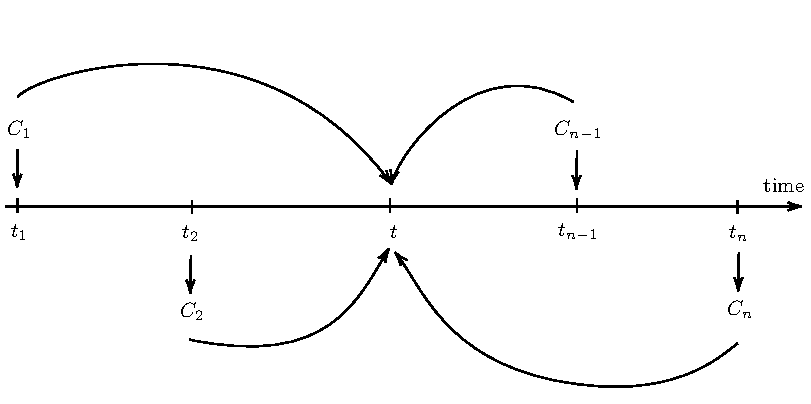
\includegraphics{SCMA329ExcelBookdownproj_files/figure-latex/tikz-ex2-1} 

}

\caption{Timeline of a series of cashflows}\label{fig:tikz-ex2}
\end{figure}

\textbf{Notes}
1. At a fixed effective rate of interest, the original series of
cashflows is equivalent to a single payment of amount \(PV(t)\) at
time \(t\).

\begin{enumerate}
\def\labelenumi{\arabic{enumi}.}
\setcounter{enumi}{1}
\tightlist
\item
  If two different series of cashflows have the same \(PV\) at one time
  at a given effective rate of interest, then they have the same \(PV\)
  at any time at that effective rate of interest.
\end{enumerate}

\hypertarget{level-annuities-certain}{%
\subsubsection{Level Annuities certain}\label{level-annuities-certain}}

An \emph{annuity} is a regular series of payments (cashflows). When the
payments are certain which are payable for a definite period of time, we
call it an \emph{annuity certain}.

\begin{itemize}
\item
  If the payments are made at the end of each time period, they are
  paid \emph{in arrear}.
\item
  Otherwise, payments are made at the beginning of each time period,
  they are pain \emph{in advance}.
\item
  An annuity paid in advance is also known as an \emph{annuity due}
\item
  If each payment is for the same amount, this is a \emph{level} annuity.
\end{itemize}

\begin{example}
\protect\hypertarget{exm:unlabeled-div-5}{}\label{exm:unlabeled-div-5}

\textbf{Example 3}. \emph{Let \(i\) be the constant effective rate of interest per
time unit. In Excel, one can calculate the accumulated value of a level
annuity certain having cashflow of pmt unit at the end of each of the
next \(n\) time units by \[\text{FV}(i\%, n, pmt, 0).\] The cashflows of
this annuity is shown in the timeline below.}

\begin{figure}

{\centering 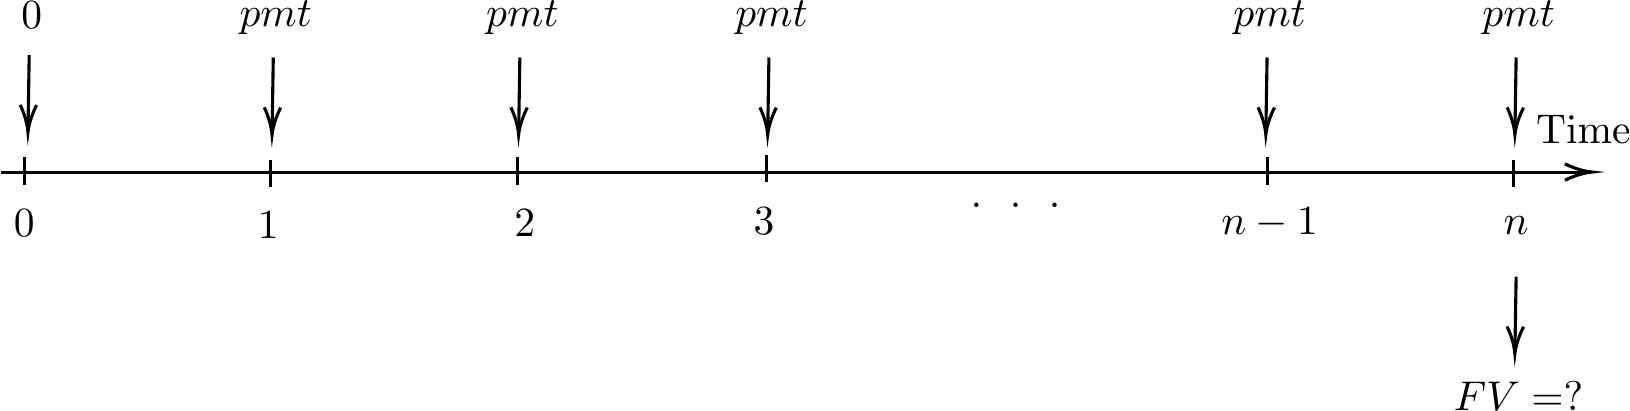
\includegraphics{SCMA329ExcelBookdownproj_files/figure-latex/tikz-ex3-1} 

}

\caption{Level Annuity Certain}\label{fig:tikz-ex3}
\end{figure}

\textbf{Note}
\emph{The last argument of the above syntax, {[}pv{]} (optional) which is an
additional cash flow now (at time 0), has been set to 0.}

\end{example}

\begin{example}
\protect\hypertarget{exm:unlabeled-div-6}{}\label{exm:unlabeled-div-6}

\textbf{Example 4}. \emph{Let \(i\) be the constant effective rate of interest per
time unit. In Excel, one can calculate the present value at time 0 of a
level annuity certain having cashflow of pmt unit at the end of each of
the next \(n\) time units by \[\text{PV}(i\%, n, pmt, 0).\]}

\end{example}

The timeline of these cashflows is shown in the figure below:

\begin{figure}

{\centering 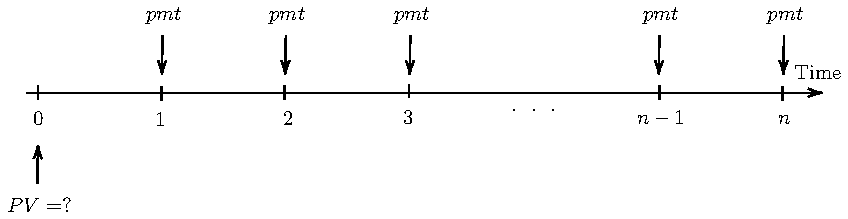
\includegraphics{SCMA329ExcelBookdownproj_files/figure-latex/tikz-ex4-1} 

}

\caption{Level Annuity Certain}\label{fig:tikz-ex4}
\end{figure}

\textbf{Note}
The last argument of the above syntax, {[}fv{]} (optional) which is an
additional cash flow at time \(n\), has been set to 0.

\begin{example}
\protect\hypertarget{exm:unlabeled-div-7}{}\label{exm:unlabeled-div-7}

\textbf{Example 5}. \emph{Given the effective rate of interest of \(8\%\) p.a., use
Excel to calculate}

\begin{enumerate}
\def\labelenumi{\arabic{enumi}.}
\item
  \emph{the accumulation at 12 years of payable yearly in arrear for the
  next 12 years.}
\item
  \emph{the present value now of ,000 payable yearly in arrear for the next
  6 years.}
\item
  \emph{the present value now of ,000 payable half-yearly in arrear for the
  next 12.5 years.}
\end{enumerate}

\end{example}

\begin{example}
\protect\hypertarget{exm:unlabeled-div-8}{}\label{exm:unlabeled-div-8}

\textbf{Example 6}. \emph{Let \(i = 4\%\) effective per time unit. Cashflows are
given as follows:}

\begin{itemize}
\item
  \emph{\(C_1 = 200\) at time \(t_1 = 1\).}
\item
  \emph{\(C_2 = 300\) at time \(t_2 = 3\).}
\item
  \emph{\(C_3 = -100\) at time \(t_3 = 5\).}
\item
  \emph{\(C_4 = -50\) at time \(t_4 = 6\).}
\end{itemize}

\emph{Develop the model using Excel to calculate}

\begin{enumerate}
\def\labelenumi{\arabic{enumi}.}
\item
  \emph{the accumulation at time \(t = 7\).}
\item
  \emph{the present value at time \(t = 0\).}
\item
  \emph{the present value at time \(t = 4\).}
\end{enumerate}

\end{example}

\begin{center}\rule{0.5\linewidth}{0.5pt}\end{center}

\hypertarget{tutorial-1}{%
\section{Tutorial 1}\label{tutorial-1}}

\begin{enumerate}
\def\labelenumi{\arabic{enumi}.}
\item
  Calculate the following accumulation:

  \begin{enumerate}
  \def\labelenumii{\arabic{enumii}.}
  \item
    Accumulate \$5,000 for 4 years at 7.5\% per annum effective.
  \item
    Accumulate \$800 for 2.7 years at 3\% per quarter-year effective.
  \item
    Accumulate \$10,000 for 27 months at 4.25\% per half-year
    effective.
  \end{enumerate}
\item
  Calculate the present values on 1 January 2015 of the following
  payments at the given rates of interest:

  \begin{enumerate}
  \def\labelenumii{\arabic{enumii}.}
  \item
    \$1,000 on 1 January 2016, at 7.5\% per annum effective.
  \item
    \$100 on 1 October 2016, at 3\% per quarter-year effective.
  \item
    \$10,000 on 1 April 2016, at 4.25\% per half-year effective.
  \end{enumerate}
\item
  \begin{enumerate}
  \def\labelenumii{\arabic{enumii}.}
  \item
    If the effective rate of interest is 4\% per annum, calculate the
    effective rate of interest per month?
  \item
    If the effective rate of interest is 6.5\% per half-year,
    calculate the effective rate of interest per quarter-year?
  \end{enumerate}
\item
  The effective rate of interest per annum was 4\% during 2015, 5\%
  during 2016 and 6\% thereafter.

  \begin{enumerate}
  \def\labelenumii{\arabic{enumii}.}
  \item
    Calculate the accumulation of \$500 from 1 January 2015 to 1
    January 2018.
  \item
    Calculate the accumulation of \$2000 from 1 April 2015 to 1
    October 2017.
  \item
    Calculate the accumulation factor from 1 January 2015 to 1
    January 2018.
  \end{enumerate}
\item
  You deposit \$ 3000 to an account that earn 2.5\% compounded
  annually. How much will you have in three years?
\item
  A person borrows a sum of \$5,000 and agrees to pay this back at the
  end of 1 year with interest calculated at an effective rate of 10\%
  per annum. Calculate the amount to be repaid for the loan.
\item
  You want to have \$1000 in 2 years and \$2000 in 4 years. How much
  should you deposit now into an account earning the effective rate of
  5.75\% semiannually?
\item
  Katy deposits 100 into a saving account which pays interest at \(i\)
  \textbf{per quarter} effective.

  At the same time, Taylor deposits 500 into a different saving
  account which pays a simple interest at an annual rate of \(i\).

  During the last 3 months of the 4th year, they both earn the same
  amount of interest. Calculate \(i\).
\item
  An ordinary annuity is a series of equal payments made at the end of
  consecutive periods over a fixed length of time. Draw a timeline for
  the following annuity having cashflow of 1 unit at the end of each
  of the next n time units.
\item
  Draw a timeline to illustrate this insurance benefit: Whole Life
  Insurance - payable immediately on death - has following conditions:

  \begin{itemize}
  \item
    death benefit (sum insured) of 1
  \item
    payable immediately on the death
  \item
    of an individual currently aged x
  \item
    for death occurring any time in the future.
  \end{itemize}
\item
  (Excel) It is a good exercise to check whether the Excel worksheet
  you have developed so far for calculating the present value and
  future value can be applied to the questions in this Tutorial. What
  would you do to improve the Excel worksheet that can be applied to a
  more general scenario?
\end{enumerate}

\hypertarget{tutorial-2}{%
\section{Tutorial 2}\label{tutorial-2}}

\begin{enumerate}
\def\labelenumi{\arabic{enumi}.}
\item
  Starting at 1 January 2015, the effective rate of interest per annum
  was 3\% per quarter-year for 9 months, 4\% per half-year for 15 months
  and and 2\% per month thereafter.

  \begin{enumerate}
  \def\labelenumii{\arabic{enumii}.}
  \item
    Calculate the accumulation factor from 1 January 2015 to 1
    January 2018.
  \item
    Calculate the accumulation of \$5,000 from 1 July 2015 to 1
    October 2017.
  \item
    Calculate the accumulation of \$100 from 1 March 2016 to 1
    August 2018.
  \item
    Calculate the present value at 1 January 2015 of \$ 25,000
    receivable on 1 July 2016.
  \item
    Calculate the present value at 1 April 2015 of \$ 8,000
    receivable on 1 October 2017.
  \item
    Calculate the discount factor from 1 July 2015 to 1
    October 2016.
  \end{enumerate}
\item
  The effective rate of interest is 7.25\% per time unit. Cashflows are
  shown in the following time line.

  \begin{enumerate}
  \def\labelenumii{\arabic{enumii}.}
  \item
    Calculate the accumulation at time time t = 4 units of these
    cashflows.
  \item
    Calculate the accumulation at time time t = 8 units of these
    cashflows.
  \item
    Calculate the present value at time time t = 0 units of these
    cashflows.
  \end{enumerate}
\end{enumerate}

\begin{center}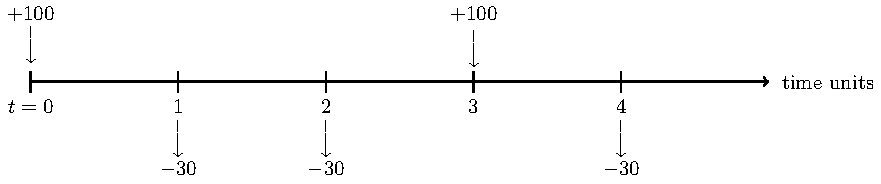
\includegraphics{SCMA329ExcelBookdownproj_files/figure-latex/tikz-ex0-1} \end{center}

\begin{enumerate}
\def\labelenumi{\arabic{enumi}.}
\setcounter{enumi}{2}
\item
  The effective rate of interest is 6\% per time unit. Cashflows are
  shown in the following time line.

  \begin{enumerate}
  \def\labelenumii{\arabic{enumii}.}
  \item
    Calculate the accumulation at time time t = 5 units of these
    cashflows.
  \item
    Calculate the value at time time t = 2 units of these cashflows.
  \item
    Calculate the present value at time time t = 0 units of these
    cashflows.
  \end{enumerate}
\end{enumerate}

\begin{center}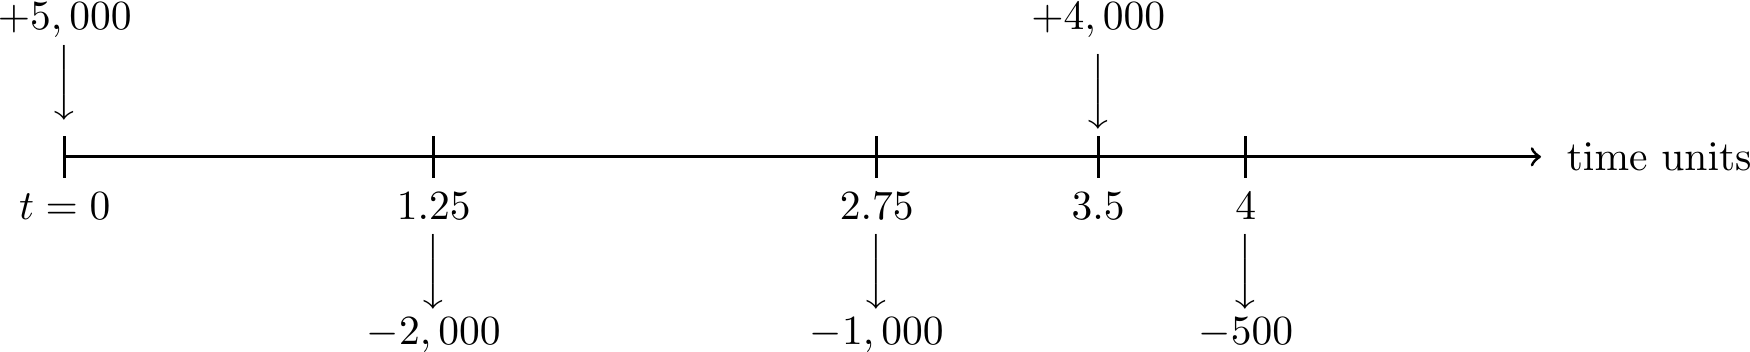
\includegraphics{SCMA329ExcelBookdownproj_files/figure-latex/tikz-ex1-1} \end{center}

\begin{enumerate}
\def\labelenumi{\arabic{enumi}.}
\setcounter{enumi}{3}
\item
  The effective rate of interest per annum was 4\% during 2015, 3\% per
  half-year until 1 October 2017 and 1.5\% per month thereafter.
  Cashflows are shown in the following time line.

  \begin{enumerate}
  \def\labelenumii{\arabic{enumii}.}
  \item
    Calculate the accumulation on 1/1/2019 of these cashflows.
  \item
    Calculate the present value on 1/1/2015 of these cashflows.
  \item
    Calculate the value at time time 1/7/2017 of these cashflows.
  \end{enumerate}
\item
  (Excel) It is a good exercise to check whether the Excel worksheet
  you have developed so far for calculating the present value and
  future value can be applied to the questions in this Tutorial. What
  would you do to improve the Excel worksheet for a more general
  scenario?
\end{enumerate}

\hypertarget{tutorial-3}{%
\section{Tutorial 3}\label{tutorial-3}}

\begin{enumerate}
\def\labelenumi{\arabic{enumi}.}
\item
  Calculate the present value now of an annuity payable monthly in
  advance. The annual amount of the annuity will be \$ 2,400 for the
  first 10 years and \$ 3,600 for the next 15 years, after which
  payment will cease. Assume that the effective rate of interest is 2\%
  per annum.
\item
  Assume that the effective rate of interest will be 3\% for 5 years
  from now, 4\% for the next 5 years and 5\% thereafter. Calculate the
  following values:

  \begin{enumerate}
  \def\labelenumii{\arabic{enumii}.}
  \item
    The present value of an annuity of \$ 1,000 per annum, payable
    in arrear for 15 years.
  \item
    The present value of an annuity due of \$ 500 per annum, payable
    at the beginning of the year for 20 years.
  \item
    The accumulation value of an increasing annuity payable yearly
    in arrear for 30 years. The first annual payment is \$ 100, and
    payments will be increase by \$ 100 each year.
  \item
    The accumulation value of an increasing annuity payable yearly
    in advance for 18 years. The first annual payment is \$ 1,000,
    and payments will be increase by 2\% each year (compound).
  \item
    The present value of an annuity of \$ 200, payable in arrear for
    10 years and deferred for 3 years.
  \end{enumerate}
\item
  You borrow \$ 240,000 from a bank to be repaid by the end of 5
  years. Assume that the interest rate is 4\% per annum. Consider the
  following four possible options for the loan to be repaid.

  \begin{enumerate}
  \def\labelenumii{\arabic{enumii}.}
  \item
    Calculate the amount of the repayments to repay if you choose to
    repay the loan as late as possible.
  \item
    You may choose to repay interest only during the 5 years term of
    loan and repay the capital at the end of the term. Calculate
    interest to be repaid and draw the timeline to illustrate the
    cashflows for the repayment of the loan.
  \item
    Calculate the amount X of level instalments to repay the loan
    which will be paid at the end of each year for 5 years and draw
    the timeline to illustrate the cashflows for the repayment of
    the loan.
  \item
    Calculate the amount Y of level instalments to repay the loan
    which will be paid at the end of each month for 5 years and draw
    the timeline to illustrate the cashflows for the repayment of
    the loan. \textbf{Instalment} is a sum of money due as one of several
    equal payments for something, spread over an agreed period of
    time.
  \end{enumerate}
\item
  A person now age 30 has received a pension from a company. When he
  retires at age 60, he will be paid on each birthday from the 60 to
  the 85th inclusive. The first annual payment will be half of his
  salary when he retires, and payments will then increase by 2\%
  compounding each year. Currently, he receive a salary of \$ 20,000
  and will increase by 3\% each year compounding in line with
  inflation. Assume that the effective rate of interest will be 4\% for
  the next 20 years and 5\% thereafter. Calculate the present value now
  of this pension.
\item
  (Excel) Use Excel worksheet you have developed so far to calculate
  the results from the questions in this Tutorial.
\end{enumerate}

\hypertarget{solutions-to-tutorial-1}{%
\section{Solutions to Tutorial 1}\label{solutions-to-tutorial-1}}

\begin{enumerate}
\def\labelenumi{\arabic{enumi}.}
\item
  The solutions to each question are as follows:

  \begin{enumerate}
  \def\labelenumii{\arabic{enumii}.}
  \tightlist
  \item
    \(5000 (1.075)^4 = 6677.345703\)
  \item
    Let \(i\%\) be the annual rate effective equivalent to \(3\%\) per quarter-effective, \(i = (1.03)^4 - 1\).
    Hence, the accumulation is
    \[800(1+i)^{2.7} = 800(1.03)^{4\times2.7} = 1100.859802.\]
  \item
    Let \(j\%\) be the monthly rate effective equivalent to \(4.25\%\) per half-year effective, \(j = (1.0425)^{2/12} - 1\).
    Hence, the accumulation is
    \[10000(1.0425)^{(2/12)\times27} = 12059.86056.\]
  \end{enumerate}
\item
  The solutions to each question are as follows:

  \begin{enumerate}
  \def\labelenumii{\arabic{enumii}.}
  \tightlist
  \item
    \(\frac{1000}{1.075} = 930.232558\).
  \item
    \(\frac{100}{(1.03)^7} = 81.309151\).
  \item
    Let \(j\%\) be the quarterly rate effective equivalent to \(4.25\%\) per half-year effective, \(j = (1.0425)^{2/4} - 1\).
    Hence, the present value is
    \[10000\times (1+j)^{-5} = 10000(1.0425)^{-(5/2)} = 9011.764643.\]
  \end{enumerate}
\item
  The solutions to each question are as follows:

  \begin{enumerate}
  \def\labelenumii{\arabic{enumii}.}
  \tightlist
  \item
    0.3274\%
  \item
    3.1988\%
  \end{enumerate}
\item
  The solutions to each question are as follows:

  \begin{enumerate}
  \def\labelenumii{\arabic{enumii}.}
  \tightlist
  \item
    500(1.04)(1.05)(1.06) =578.76
  \item
    \(2000(1.04)^{3/4}(1.05)(1.06)^{3/4} =2259.299\)
  \item
    (1.04)(1.05)(1.06) = 1.15752
  \end{enumerate}
\item
  The account balance in 3 years is \(3000(1.025)^{3} = 3230.67\).
\item
  The amount to be repaid for the loan is 5000(1.1) = 5500.
\item
  Let \(X\) be the amount to be deposited now.
  \[X = \frac{1000}{(1.0575)^4} + \frac{2000}{(1.0575)^8} = 2078.36. \]
\item
  At time 3.75 years, Katy has a balance of \(100(1+i)^{15}\). The interest on this balance over the next 3 months is \(100(1+i)^{15}\cdot i\).
  Taylor earns simple interest on the original amount which is equal to \(500i\cdot\frac{3}{12}\). Therefore, we solve for \(i\) from the following equation:
  \[ 100(1+i)^{15}\cdot i = 500i\cdot\frac{3}{12},\] which gives \(i = 0.014987.\)
\item
  The timeline for the following annuity having cashflow of 1 unit at the end of each of the next \(n\) time units is given in the figure below:
\end{enumerate}

\begin{center}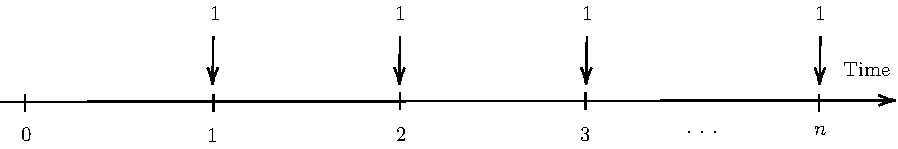
\includegraphics{SCMA329ExcelBookdownproj_files/figure-latex/tikz-sol1-1} \end{center}

\begin{enumerate}
\def\labelenumi{\arabic{enumi}.}
\setcounter{enumi}{9}
\tightlist
\item
  (More details in the course ``Life Contingencies I''). We need to define a random variable \(T_x\) = the remaining future life time of a life aged \(x\).
\end{enumerate}

\begin{center}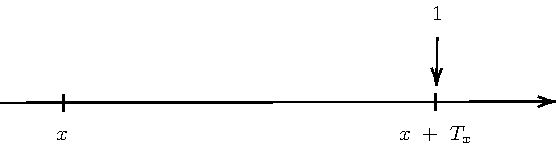
\includegraphics{SCMA329ExcelBookdownproj_files/figure-latex/tikz-sol2-1} \end{center}

The quantity of interest is the present value of the death benefit assuming the interest rate of \(i\%\) p.a. effective. It is also a random variable,
\[PV = \frac{1}{(1+i)^{T_x}}.\] It turns out that the premium rate of this whole life insurance is \(E[PV]\), the expected value of the present value, \(PV\).

\hypertarget{solutions-to-tutorial-2}{%
\section{Solutions to Tutorial 2}\label{solutions-to-tutorial-2}}

\begin{enumerate}
\def\labelenumi{\arabic{enumi}.}
\item
  The solutions to each question are as follows:

  \begin{enumerate}
  \def\labelenumii{\arabic{enumii}.}
  \tightlist
  \item
    \((1.03)^3(1.04)^{2.5} (1.02)^{12} = 1.528611\)
  \item
    \(5000A(0.5,2.75) = 5000(1.03)(1.04)^{2.5} (1.02)^{9} = 6788.786068\)
  \item
    We first find the rate \(j\%\) per month effective that is equivalent to the rate of \(4\%\) per half-year effective.
    \[j = (1.04)^{1/6} - 1 = 0.00656.\]
    The accumulated value is \(100A(1+2/12, 3 + 7/12 ) = 100(1+j)^{10}(1.02)^{19} = 155.522118.\)
  \item
    \(25000V(0,1.5) = \frac{25000}{(1.03)^3(1.04)^{1.5}} = 21571.39968.\)
  \item
    \(8000V(0.25,2.75) = \frac{8000}{(1.03)^2(1.04)^{2.5}(1.02)^{9}} = 5720.455921.\)
  \item
    \(V(0.5,1.75) = \frac{1}{(1.03)(1.04)^{2}} = 0.897627.\)
  \end{enumerate}
\item
  The solutions to each question are as follows:

  \begin{enumerate}
  \def\labelenumii{\arabic{enumii}.}
  \tightlist
  \item
    With \(i = 7.25\%\) per time period, \(V(4) = 100 (1+i)^4 - 30(1+i)^3 - 30 (1+i)^2 + 100 (1+i) - 30 = 138.041762.\)
  \item
    \(V(8) = V(4)\cdot (1+i)^4 = 182.641597.\)
  \item
    \(PV(0) = V(4)\cdot (1+i)^{-4} = 104.332903.\)
  \end{enumerate}
\item
  The solutions to each question are as follows:

  \begin{enumerate}
  \def\labelenumii{\arabic{enumii}.}
  \tightlist
  \item
    With \$ = 6\%\$ per time period, \(V(5) = 5000 (1+i)^5 - 2000(1+i)^{3.75} - 1000 (1+i)^{2.25} + 4000 (1+i)^{1.5} - 500(1+i) = 6897.948585.\)
  \item
    \(V(2) = V(5)(1+i)^{-3} = 5791.650645.\)
  \item
    \(PV(0) = V(5)(1+i)^{-5} = 5154.548456.\)
  \end{enumerate}
\item
  The solutions to each question are as follows:

  \begin{enumerate}
  \def\labelenumii{\arabic{enumii}.}
  \tightlist
  \item
    \(V(1/1/2019) = 100(1.04)(1.03)^{3.5}(1.015)^{15} - 30 (1.03)^{3.5} (1.015)^{15}- 30 (1.03)^{1.5} (1.015)^{15} + 100 (1.015)^{12} - 30 = 152.955693.\)
  \item
    \(PV(0)= V(1/1/2015) = \frac{152.955693}{(1.04)(1.03)^{3.5}(1.015)^{15}} =106.074596.\)
  \item
    \(V(1/7/2017) = PV(0)(1.04)(1.03)^3 = 120.546998.\)
  \end{enumerate}
\end{enumerate}

\hypertarget{solutions-to-tutorial-3}{%
\section{Solutions to Tutorial 3}\label{solutions-to-tutorial-3}}

\begin{enumerate}
\def\labelenumi{\arabic{enumi}.}
\tightlist
\item
  Let \(j\) be the effective rate per month equivalent to \(i = 2\)\%. We have
  \[ j = (1.02)^{1/12}  - 1= 0.001652. \]
  Hence,
\end{enumerate}

\[ PV(0) = 200 \ddot{a}^{j}_{120} + 300 \ddot{a}^{j}_{180} \left( \frac{1}{1.02} \right)^{10} = 60148.03. \]

\begin{enumerate}
\def\labelenumi{\arabic{enumi}.}
\setcounter{enumi}{1}
\item
  The solutions to each question are as follows:

  \begin{enumerate}
  \def\labelenumii{\arabic{enumii}.}
  \item
    The cashflows have been splitted into three periods: (a) from time point 0-5, (b) 5-10 and (c) time point 10 onward.
    \[PV(0) = 1000 ( a^{3\%}_{5} + 1.03^{-5} a^{4\%}_{5} +  1.03^{-5} 1.04^{-5} a^{5\%}_{5}) = 11489.49  \]
  \item
    We have
    \[PV(0) = 500 ( \ddot{a}^{3\%}_{5} + 1.03^{-5} \ddot{a}^{4\%}_{5} +  1.03^{-5} 1.04^{-5} \ddot{a}^{5\%}_{10}) = 7229.67  \]
  \item
    The accumuated value is
    \[100 (Is)^{3\%}_{5} (1.04)^5 (1.05)^{20} + \left[100 (Is)^{4\%}_{5} + 500 s^{4\%}_{5} \right] (1.05)^{20}  + \left[100 (Is)^{5\%}_{20} + 1000 s^{5\%}_{20} \right]= 78929.01  \]
  \item
    Let \(i_1 = 3\%, i_2 = 4\%\) and \(i_3 = 5\%\). The accumuated value is given by

    \begin{aligned} 
     V(18) &= \left[1000(1+i_1)^5 + 1000(1.02)(1+i_1)^4 + 1000(1.02)^2(1+i_1)^3 + \ldots + 1000(1.02)^4(1+i_1)\right](1.04)^5(1.05)^8   \\
     &+ \left[1000(1.02)^5(1+i_2)^5 + 1000(1.02)^6(1+i_2)^4 + 1000(1.02)^7(1+i_2)^3 + \ldots + 1000(1.02)^9(1+i_2)\right](1.05)^8   \\
     &+ \left[1000(1.02)^{10}(1+i_3)^8 + 1000(1.02)^{11}(1+i_3)^7 + 1000(1.02)^{12}(1+i_3)^6 + \ldots + 1000(1.02)^{17}(1+i_3)\right]  \\
     &= 1000(1.02)^5 \left[ \left(\frac{1+i_1}{1.02}\right)^5   + \left(\frac{1+i_1}{1.02}\right)^4 + \ldots + \left(\frac{1+i_1}{1.02}\right) \right](1.04)^5(1.05)^8 \\
     &+ 1000(1.02)^{10} \left[ \left(\frac{1+i_2}{1.02}\right)^5   + \left(\frac{1+i_2}{1.02}\right)^4 + \ldots + \left(\frac{1+i_2}{1.02}\right) \right](1.05)^8 \\
      &+ 1000(1.02)^{18} \left[ \left(\frac{1+i_3}{1.02}\right)^8   + \left(\frac{1+i_3}{1.02}\right)^7 + \ldots + \left(\frac{1+i_3}{1.02}\right) \right] 
     \end{aligned}

    Let \(1+j_1 = \frac{1+i_1}{1.02}\). Then, \(j_1 = 0.009804\) and
    \[ \left[ \left(\frac{1+i_1}{1.02}\right)^5   + \left(\frac{1+i_1}{1.02}\right)^4 + \ldots + \left(\frac{1+i_1}{1.02}\right) \right] = \frac{(1+j_1)^5 - 1}{j_1/(1+j_1)} = 5.148995.\]
    Let \(1+j_2 = \frac{1+i_2}{1.02}\). Then, \(j_2 = 0.019608\) and
    \[ \left[ \left(\frac{1+i_2}{1.02}\right)^5   + \left(\frac{1+i_2}{1.02}\right)^4 + \ldots + \left(\frac{1+i_2}{1.02}\right) \right] = 5.301921.\]
    Let \(1+j_3 = \frac{1+i_3}{1.02}\). Then, \(j_3 = 0.029412\) and
    \[ \left[ \left(\frac{1+i_3}{1.02}\right)^8   + \left(\frac{1+i_3}{1.02}\right)^7 + \ldots + \left(\frac{1+i_3}{1.02}\right) \right]  = 9.134790.\]
    Therefore, \(V(18) = 32814.45\).
  \item
    The present value is
  \end{enumerate}
\end{enumerate}

\begin{aligned}
    PV(0) &= \left( \frac{200}{(1.03)^4} + \frac{200}{(1.03)^5}\right) + 200 a^{0.04}_5 (1.03)^{-5} + 200 a^{0.05}_{3} (1.03)^{-5} (1.04)^{-5} \\
    &= 350.2192 + 768.0362 + 386.1574 = 1504.413
\end{aligned}

\begin{enumerate}
\def\labelenumi{\arabic{enumi}.}
\setcounter{enumi}{2}
\item
  The solutions to each question are as follows:

  \begin{enumerate}
  \def\labelenumii{\arabic{enumii}.}
  \tightlist
  \item
    \(240000 (1.04)^5 = 291996.7\)
  \item
    The interest amounts are \(0.04\times 240000 = 9600.\)
  \item
    By the Principle of Equivalence, we have
    \[ 240000 = X a^{0.04}_{5}. \]
    This gives X = 53910.51.
  \item
    Level installments are payable monthly, which follows
    \[ 240000 = Y a^{j}_{60}, \]
    where \(j = (1.04)^{1/12} - 1\). This gives Y = 4412.23.
  \end{enumerate}
\item
  The person retires in 30 years, when his salary is expected to be
  \(20000 \times (1.03)^{30} = 48545.25.\)
  The first payment will be half of this which is equal to 24272.62.
  The present value at age 60 of his pension is
  \[  24272.62 \times \ddot{a}^{0.029412}_{26} = 449717.9\] (the precise value is 449719.051954).
  Here we use \(\frac{1.05}{1.02} = 1.029412\) and the annuity is paid from the 60th to the 85th birthday inclusive so there are 26 payments made in advance.
  Therefore, the present value of this at age 30 is
  \[ 449717.9 \times (1.05)^{-10} \times (1.04)^{-20} = 126002.9. \]
  (the precise value is 126003.181173)
\end{enumerate}

\end{document}
